En este capítulo se mostrarán algunos de los informes que genera la aplicación, tanto en pdf como csv.

\section{Horarios}

Se puede exportar un horario completo a CSV, se muestran en el mismo archivo separados por saltos de línea los horarios pertenecientes a un grupo. Un ejemplo sería el siguiente:

\begin{verbatim}
Horario tipo 
,L,M,X,J,V
09:00,"ADAI C3",,,"pI A2","pI A2"
09:30,"ADAI C3",,"ADAI C4","pI A2","pI A2"
10:00,"ADAI C3",,"ADAI C4",,
10:30,"ADAI C3",,"ADAI C4","pI A2",
11:00,,,"ADAI C4",,"ADAI B4"
11:30,"pI B2","pI A2",,,"ADAI B4"
12:00,"pI B2",,,,"ADAI B4"
12:30,"pI B2",,,,"ADAI B4"
13:00,"pI B2",,,"ADAI A2","ADAI B4"
13:30,,,,,"ADAI B4"
14:00,,"ADAI A2",,"ADAI B6",
14:30,"ADAI B5",,,"ADAI B6","ADAI A2"
15:00,"ADAI B5",,,"ADAI B6","ADAI A2"
15:30,"ADAI B5",,,"ADAI B6","ADAI A2"
16:00,"ADAI B5",,,"ADAI B6",
16:30,"ADAI B5",,,"ADAI B6","ADAI A2"
17:00,"ADAI B5",,,,
17:30,,,,,
18:00,,,,,
18:30,,,,,
19:00,,,,,
19:30,,,,,
20:00,,,,,
20:30,,,,,
21:00,,,,,
21:30,,,,,
22:00,,,,,

Semana 1
,L,M,X,J,V
09:00,,,,"pI A2","pI A2"
09:30,,,,"pI A2","pI A2"
10:00,,,,,
10:30,,,,"pI A2",
11:00,,,,,
11:30,,,,,
12:00,,,,,
12:30,,,,,
13:00,,,,"ADAI A2",
13:30,,,,,
14:00,,,,"ADAI A2",
14:30,,,,,"ADAI A2"
15:00,,,,,"ADAI A2"
15:30,,,,"pI A2","ADAI A2"
16:00,,,,,
16:30,,,,,"ADAI A2"
17:00,,,,,
17:30,,,,,
18:00,,,,,
18:30,,,,,
19:00,,,,,
19:30,,,,,
20:00,,,,,
20:30,,,,,
21:00,,,,,
21:30,,,,,
22:00,,,,,

Semana 3
,L,M,X,J,V
09:00,,,,"pI A2","pI A2"
09:30,,,,"pI A2","pI A2"
10:00,,,,,
10:30,,,,"pI A2",
11:00,,,,,
11:30,,"pI A2",,,
12:00,,,,,
12:30,,,,,
13:00,,,,"ADAI A2",
13:30,,,,,
14:00,,"ADAI A2",,,
14:30,,,,,"ADAI A2"
15:00,,,,,"ADAI A2"
15:30,,,,,"ADAI A2"
16:00,,,,,
16:30,,,,,"ADAI A2"
17:00,,,,,
17:30,,,,,
18:00,,,,,
18:30,,,,,
19:00,,,,,
19:30,,,,,
20:00,,,,,
20:30,,,,,
21:00,,,,,
21:30,,,,,
22:00,,,,,

Semana 2
,L,M,X,J,V
09:00,,,,"pI A2","pI A2"
09:30,,,,"pI A2","pI A2"
10:00,,,,,
10:30,,,,"pI A2",
11:00,,,,,
11:30,,"pI A2",,,
12:00,,,,,
12:30,,,,,
13:00,,,,"ADAI A2",
13:30,,,,,
14:00,,"ADAI A2",,,
14:30,,,,,"ADAI A2"
15:00,,,,,"ADAI A2"
15:30,,,,,"ADAI A2"
16:00,,,,,
16:30,,,,,"ADAI A2"
17:00,,,,,
17:30,,,,,
18:00,,,,,
18:30,,,,,
19:00,,,,,
19:30,,,,,
20:00,,,,,
20:30,,,,,
21:00,,,,,
21:30,,,,,
22:00,,,,,
\end{verbatim}

Esto puede parecer desordenado, pero si se abre con un programa de edición de hojas de cálculo, como por ejemplo {\em LibreOffice}, lo veremos de la siguiente manera:


\begin{figure}[H] 
  \label{informes-horario} 
	\begin{center}
    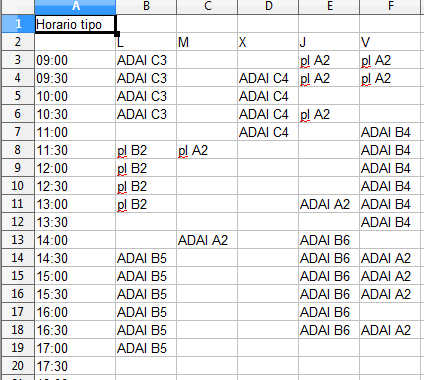
\includegraphics[scale=1]{./horario-export.png}
  \end{center}
\caption{Fragmento de un horario exportado abierto con LibreOffice Calc}
\end{figure}

Se puede observar el horario de forma bastante clara, y desde aquí podremos hacer las ediciones que veamos necesarias.

\section{Ocupación de aulas}

La ocupación de aulas se visualiza en un formato muy similar a la del horario ya que en realidad es un horario en sí mismo, pero filtrado por aula en lugar de un grupo de teoría de una titulación. La única diferencia es que solo veremos la ocupación de la semana que se haya exportado y no las tres en el mismo archivo como pasa con los horarios.
\\
Un ejemplo es el siguiente:
\begin{verbatim}
,L,M,X,J,V
09:00,"ADAI C3",,,"pI A2","pI A2"
09:30,"ADAI C3",,"ADAI C4","pI A2","pI A2"
10:00,"ADAI C3",,"ADAI C4","ADAI C1",
10:30,"ADAI C3","ADAI A1","ADAI C4","pI A2|ADAI C1",
11:00,"ADAI A1","ADAI B1","ADAI C4","ADAI C1","ADAI B4"
11:30,"pI B2","pI A2|ADAI B1",,"ADAI C1","ADAI B4"
12:00,"pI B2","ADAI B1","ADAI B2",,"ADAI B4"
12:30,"pI B2","ADAI B1","ADAI B2",,"ADAI B4"
13:00,"pI B2","ADAI B1","ADAI B2","ADAI A2","ADAI B4"
13:30,,"ADAI B1","ADAI B2",,"ADAI B4"
14:00,,"ADAI A2","ADAI B2","ADAI B6",
14:30,"ADAI B5",,"ADAI B2","ADAI B6","ADAI A2"
15:00,"ADAI B5",,,"ADAI B6","ADAI A2"
15:30,"ADAI B5",,,"ADAI B6","ADAI A2"
16:00,"ADAI B5",,,"ADAI B6",
16:30,"ADAI B5",,,"ADAI B6","ADAI A2"
17:00,"ADAI B5",,,,
17:30,,,,,
18:00,,,,,
18:30,,,,,
19:00,,,,,
19:30,,,,,
20:00,,,,,
20:30,,,,,
21:00,,,,,
21:30,,,,,
22:00,,,,,
\end{verbatim}

Visualizado desde {\em LibreOffice Calc} se vería como en la siguiente imagen:

\begin{figure}[H] 
  \label{informes-ocupacion} 
	\begin{center}
    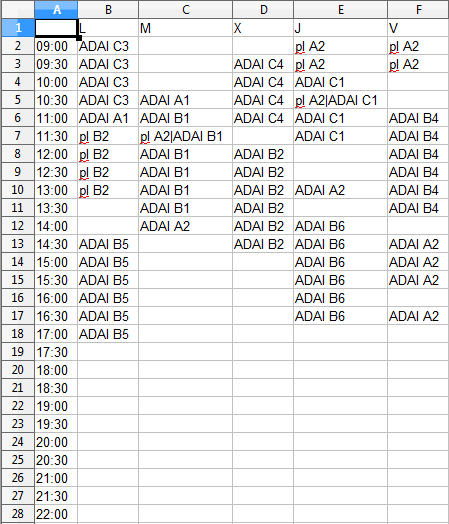
\includegraphics[scale=1]{./aula-export.png}
  \end{center}
\caption{Fragmento de la ocupación de un aula exportada abierta con LibreOffice Calc}
\end{figure}

\section{Informes de asignatura}
 
Podemos hacer informes de asignaturas en PDF con las horas que se impartirán cada semana según los horarios, el PDF se visualizará como el de la siguiente imagen:

\begin{figure}[H] 
  \label{informes-asignatura} 
	\begin{center}
    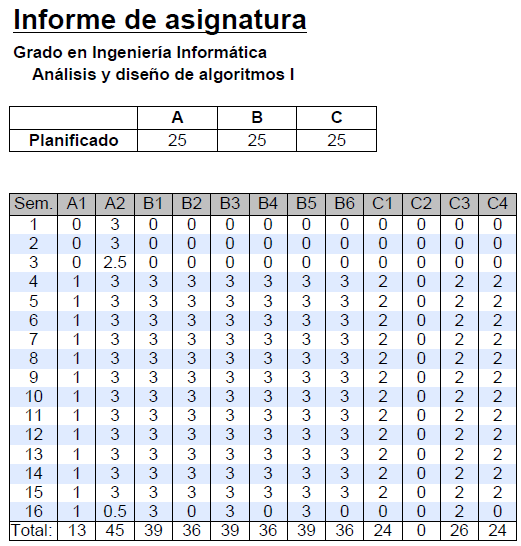
\includegraphics[scale=1]{./informe-pdf-asignatura.png}
  \end{center}
\caption{Fragmento un informe PDF de una asignatura}
\end{figure}

\section{Calendario}

En la sección de eventos podemos hacer una exportación completa del calendario del curso al formato CSV. Debido a la dificultad por encontrar un formato adecuado, se ha optado por separar cada mes, y en cada casilla del fichero CSV, incluir un día del mes, con cada semana en cada línea.
\\
Para marcar los eventos, en lugar de poner el número del día, se marca la casilla con una X, también estarán marcados con una X, al no ser lectivos, los sábados y domingos, y los días previos o posteriores a inicio y final de curso respectivamente. 
\\
Se marcan con un guión las casillas sobrantes en cada mes que no corresponden con ningún día de ese mes.
\\
A continuación se puede ver un calendario con algunos eventos de prueba marcados para mostrar el formato en el que se exporta:

\begin{verbatim}
"Semestre 1"
"Mes 9"
X,X,X,22,23,X,X
26,27,28,29,30,-,-
"Mes 10"
-,-,-,-,-,X,X
03,04,05,06,07,X,X
10,11,12,13,14,X,X
17,18,19,20,21,X,X
24,25,26,27,28,X,X
31,-,-,-,-,-,-
"Mes 11"
-,01,02,03,04,X,X
07,08,09,10,11,X,X
14,15,16,X,18,X,X
21,22,23,24,25,X,X
28,29,30,-,-,-,-
"Mes 12"
-,-,-,01,02,X,X
05,06,07,08,09,X,X
12,13,14,15,16,X,X
19,20,21,22,23,X,X
26,27,28,29,30,X,-
"Mes 1"
-,-,-,-,-,-,X
02,03,04,05,06,X,X
X,X,X
"Semestre 2"
"Mes 2"
X,14,15,16,17,X,X
20,21,22,X,24,X,X
X,X,X,-,-,-,-
"Mes 3"
-,-,-,01,02,X,X
05,06,07,08,09,X,X
12,13,14,15,16,X,X
19,20,21,22,23,X,X
26,27,28,29,30,X,-
"Mes 4"
-,-,-,-,-,-,X
02,03,04,05,06,X,X
09,10,11,12,13,X,X
16,17,18,19,20,X,X
23,24,25,26,27,X,X
30,-,-,-,-,-,-
"Mes 5"
-,01,02,03,04,X,X
07,08,09,X,11,X,X
14,15,16,17,18,X,X
21,22,23,24,25,X,X
28,29,30,31,-,-,-
"Mes 6"
-,-,-,-,01,X,X
04,05,06,07,08,X,X

\end{verbatim}
